\section{Broadcast: protocols and additional measurements}
\label{app:audit}\label{app:rd}
This appendix gives the experimental details for \cref{sec:broadcast}. We examine how OPD changes prefix visitation and the student's predictions on fixed prefixes. We then ask whether the student can complete its reasoning from those prefixes and reach a correct answer. The theoretical backbone is derived and presented in \cref{app:rd-flow,app:broadcast-prefix-reweighting,app:rd-theory,app:outcome-proof,app:rd-entropy-response}.

\subsection{Models and measurement setup}
\label{app:rd-protocol}

\paragraph{Models and training.}
All three learners use JustRL-1.5B as the teacher. The strong learner is DeepSeek-R1-Distill-Qwen-1.5B which we also studied in \cref{sec:conversion}. The unprepared learner is Qwen2.5-1.5B-Instruct. ``Prepared Qwen'' starts from the same Qwen 1.5B instruct model after four passes of offline distillation on OpenMathInstruct2 (see the preparation section, \cref{app:preparation} for more details). The Qwen runs use 200 training steps, 256 rollouts per update, temperature 1.0, and an 8,192-token generation cap. DeepSeek's generation cap is 4,096 tokens.

\paragraph{Rollout banks.}
We save 32 rollouts from each batch $\ell\in\{1,21,41,\ldots,161,181,196\}$. A bank is this fixed set of rollout texts. Batch $\ell$ is generated after $\ell-1$ updates. Thus batch 41 appears at update 40 in the routing and drift plots. Checkpoint 0 is each learner's starting model, including the offline-prepared model for prepared Qwen.


\paragraph{When does the model initiate checking?}
The WAIT family $\mathcal W$ contains the 13 tokens that decode to ``wait'' (after whitespace is removed and text is lowercased). We examine candidate sentence starts: the first response position and positions after a token ending in a period, question mark, exclamation mark, colon, or newline. The student and teacher probabilities of this family are denoted as $w_t(x)=p_t(\mathcal W\mid x)$ and $q_W(x)=q(\mathcal W\mid x)$. We measure the mean $\log w_t$ across candidate starts. For the above- and below-teacher comparisons, we use log-odds $b_t=\log[w_t/(1-w_t)]$ and $b_q=\log[q_W/(1-q_W)]$.

We form the two groups using a reference checkpoint $r$: checkpoint 0 for DeepSeek and checkpoint 20 for the Qwen learners. We include a prefix only if $\max(w_r,q_W)\ge10^{-3}$ and $|b_r-b_q|\ge0.5$. The sign of $b_r-b_q$ determines whether the student initially assigns more or less probability than the teacher. Each prefix keeps the same group at every evaluated checkpoint.

We also count emitted WAIT tokens per thousand response tokens, and measure the arithmetic mean of $w_t$ at candidate starts. These quantities answer different questions. The emission rate counts what the model actually generates. Mean probability and mean log probability describe its actual predictions at the selected prefixes. 

To assess agreement with the teacher, we use the binary discrepancy $c_W=\KL{\operatorname{Ber}(q_W)}{\operatorname{Ber}(w_t)}$. At a fixed prefix, $\partial_t c_W=(w_t-q_W)\partial_t b_t$. Lowering WAIT probability improves agreement only while the student's probability is above the teacher's. 


\begin{table}[ht]
\centering\small
\setlength{\tabcolsep}{4pt}
\begin{tabular}{lrrrrrrrr}
\toprule
&\multicolumn{4}{c}{Local loss}&\multicolumn{4}{c}{Conditional entropy}\\
\cmidrule(lr){2-5}\cmidrule(lr){6-9}
Learner & Initial & Final & $\sum\widehat R$ & $\sum\widehat D$ & Initial & Final & $\sum\widehat R$ & $\sum\widehat D$\\
\midrule
DeepSeek & 0.263 & 0.015 & -0.033 & -0.214 & 0.664 & 0.707 & -0.049 & 0.093\\
Unprepared & 0.579 & 0.073 & 0.474 & -0.980 & 0.650 & 3.988 & 3.666 & -0.327\\
Prepared & 0.707 & 0.362 & 0.108 & -0.453 & 2.171 & 0.842 & -1.183 & -0.146\\
\bottomrule
\end{tabular}
\caption{\textbf{Cumulative routing and drift contributions to loss and entropy.} The comparisons run from initialization through batch 161, including evaluations at substitute checkpoints. Values are rounded independently. At full precision, the routing and drift contributions sum to the change from the initial to the final mean.}\label{tab:rd-summary}
\end{table}

\subsection{DeepSeek: adjusting the probability of checking}
\label{app:rd-checking}

DeepSeek's local loss falls mainly because its predictions change at fixed prefixes (\cref{tab:rd-summary}). We next ask whether these changes bring its checking probabilities closer to the teacher's, as``wait''-initiated checking / backtracking is a dominant part of the model's reasoning traces and observed to initiate sentences in which the model manage its epistemic states \citep{marjanovic2026deepseekr}. We use the classes in \cref{app:rd-protocol}, defined by whether the reference student's WAIT probability lies above or below the teacher's.

In the first 512 tokens, the above-teacher class has $\sum\widehat R=0.036$ and $\sum\widehat D=-1.824$. The below-teacher class has $0.505$ and $1.918$, respectively. The drift contribution therefore lowers mean checking log-odds in the first class and raises them in the second. The main plot uses filled circles and open triangles for these two classes. Routing can still be large within individual intervals, even when its contributions partly cancel over training.

We check whether this two-sided adjustment reduces the discrepancy from the teacher on a fixed set of prefixes (\cref{tab:rd-check-calibration}). For DeepSeek, the discrepancy falls from $0.0789$ to $0.0032$ in the above-teacher class and from $0.1915$ to $0.0149$ in the below-teacher class. Interestingly, the same comparison on held-out prepared-Qwen text gives decreases from about $0.039$ to $0.014$ and from $0.293$ to $0.039$, so the improvement even extends beyond DeepSeek's own generated prefixes.

To examine how closely the changes follow the teacher, we regress the change in student log-odds on the teacher and reference-student log-odds. On DeepSeek's own prefixes at checkpoint 200, the teacher coefficient is about $0.90$, the reference-student coefficient about $-0.88$, and $R^2$ about $0.94$. This detailed relation is much weaker on the held-out Qwen prefixes. The fixed-prefix results support improved calibration on both sets, but the closer match to the teacher's pattern occurs on DeepSeek's own text.

\begin{table}[ht]
\centering\small
\begin{tabular}{llrrrr}
\toprule
Learner & Reference class & Positions & $c_W$ at reference & $c_W$ at 200 & $\Delta$ log-odds\\
\midrule
DeepSeek & Above teacher & 33,010 & 0.0789 & 0.0032 & -2.073\\
DeepSeek & Below teacher & 11,336 & 0.1915 & 0.0149 & +1.381\\
Prepared Qwen & Above teacher & 25,794 & 0.0276 & 0.0580 & -0.606\\
Prepared Qwen & Below teacher & 18,211 & 0.5627 & 0.3813 & +0.721\\
\bottomrule
\end{tabular}
\caption{\textbf{Checking probability on fixed prefixes.} We report discrepancy from the teacher, $c_W$, and the change in log-odds from the reference checkpoint to checkpoint 200. The reference is checkpoint 0 for DeepSeek and checkpoint 20 for prepared Qwen. Each class contains the same prefixes at both checkpoints. The main-text routing and drift plots instead compare successive banks.}\label{tab:rd-check-calibration}
\end{table}


\begin{figure}[ht]
\centering
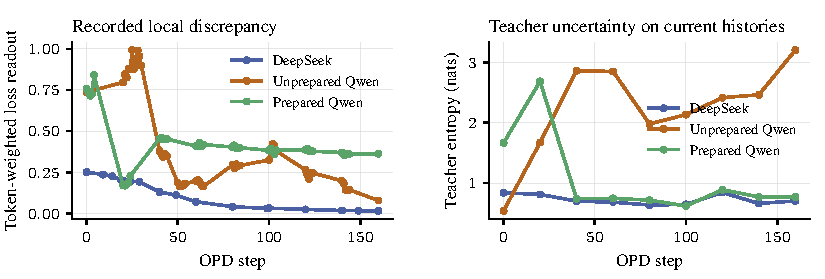
\includegraphics[width=\linewidth]{figures/section33/rd_support_overview.pdf}
\caption{\textbf{Local agreement and teacher uncertainty.} Left: local loss averaged over tokens in the full recorded batches, through the period with fixed prompt-language composition. Right: teacher entropy on the 32-rollout samples from each batch. Colors match \cref{fig:rd-contrast,fig:rd-prepared}. The teacher is generally less uncertain on DeepSeek and prepared-Qwen prefixes than on unprepared-Qwen prefixes.}
\label{fig:rd-support-overview}
\end{figure}

\subsection{Unprepared Qwen 1.5B: fitting on changing prefixes}
\label{app:rd-failure}

For unprepared Qwen, the local loss decreases ($0.579\to0.073$). The accumulated contributions are $\sum\widehat R_L=+0.474$ and $\sum\widehat D_L=-0.980$. Thus changes in predictions at fixed prefixes account for the decrease, while changes in prefix visitation raise the loss. This balance varies during training. In the first comparison at step 20, loss rises by $+0.268$: routing contributes $+0.455$, which exceeds the decrease from drift, $-0.187$. Later on, loss mainly falls through changes dominated by drift, as the main text already pointed out. The large rise in entropy has a different origin: it comes mainly from prefix visitation, as shown in the main text. 



\subsubsection{Loss and entropy on the same prefixes}
\label{app:rd-entropy-evidence}
The preceding comparisons use batches generated at different training steps. We now hold the prefixes fixed to see what the student learns on the same text. We use the prefixes from batch 41. (The entropy-response identity, how it can change through routing without significant drift, and examples are discussed in the theory presented in \cref{app:rd-entropy-response}.)

On these prefixes, student entropy falls from $4.987$ nats at initialization to $3.989$ at checkpoint 160. The local loss falls from $0.789$ to $0.057$. Teacher entropy is $2.859$ nats, below both student values. The teacher is more uncertain here than on the coherent initial text, but the student still learns sharper predictions on these prefixes.

These measurements answer different questions. The falling loss shows fitting at fixed prefixes. The entropy decomposition shows that the large rise in uncertainty mainly reflects which prefixes the model visits. Note that these are primarily examinations of how the local per-prefix readouts change. To understand how the learnt model's continuations reach a correct answer we need to probe their continuation advantages which involve non-local readouts, as \cref{eq:rd-value-rate} shows. We examine this next.

\FloatBarrier
\Needspace{10\baselineskip}
\subsection{Continuation value at the unprepared student's answer boundaries}
\label{app:steer-probe}
We now examine prefixes at which the initial student was about to answer. Holding these prefixes fixed lets us ask two questions: how does training change the probability of answering now, and how successful are the continuations from the two alternatives? This comparison isolates changes at the selected prefixes from changes in prefix visitation.

\paragraph{Prefix selection and continuation conditions.}
We sample two rollouts per problem from the initial student on 50 held-out MATH-500 problems. ``Cutting'' the rollout immediately before a final-answer marker (\texttt{\textbackslash boxed} or \texttt{Answer:}) gives 86 prefixes. We evaluate the initial student, checkpoints 20--200 of the unprepared run, and the JustRL teacher on these same prefixes. For each model, we record the next-token probability mass $\pi$ on the probe's answer class.

We draw six continuations per prefix under each of \emph{three conditions}: the \emph{answer} condition forces the answer token, the ``continue'' condition forces the model's most probable non-answer token, and the ``natural'' condition samples without forcing either token. All conditions use temperature $0.6$, \mbox{top-$p=0.95$}, and a cap of $16{,}384$ new tokens. \Cref{tab:steer-probe} reports the fraction of correct continuations.

\paragraph{Branch probabilities and continuation values.}
Let $Q_{\rm ans}$ and $Q_{\rm cont}$ denote the correctness values of the two forced branches, ``answer'' vs ``continue'' (recall that $Q$ denotes the continuation success rate from the given prefix distribution after forcing an action choice). Their probability-weighted probe value is $V=\pi Q_{\rm ans}+(1-\pi)Q_{\rm cont}$. This value's change relative to the initial student decomposes as
\[
\Delta V=
\underbrace{\Delta\pi\,(\bar Q_{\rm ans}-\bar Q_{\rm cont})}_{\text{changed branch probability}}
+\underbrace{\bar\pi\,\Delta Q_{\rm ans}+(1-\bar\pi)\,\Delta Q_{\rm cont}}_{\text{changed branch values}},
\]
where bars denote the average of the two endpoint values at the same prefix. The first term describes moving probability between the two branches. It is positive when probability moves \emph{toward} the more successful branch. The second term describes changes in the branch continuation values. We calculate both terms at each prefix before averaging, and obtain intervals from $2{,}000$ bootstrap draws over prefixes. Note that this split applies to the two forced branches. The most probable non-answer token can differ between models. The continue-branch value therefore includes both that first choice and the later continuation. Natural continuations are sampled separately, and their success rate need not equal $V$.

\begin{table}[htb]
\centering\small\setlength{\tabcolsep}{4pt}
\begin{tabular}{lrrrrrrr}
\toprule
 & log-odds of & \multicolumn{3}{c}{correctness} & \multicolumn{3}{c}{change in two-branch value}\\
\cmidrule(lr){3-5}\cmidrule(lr){6-8}
Evaluator & answering & answer & continue & natural & $\Delta V$ & probability term & value term\\
\midrule
initial student & $+2.4$ & 0.30 & 0.22 & 0.27 & --- & --- & ---\\
update 20  & $-3.9$ & 0.30 & 0.29 & 0.29 & $+0.01$ & $-0.03$ & $+0.05$\\
update 30  & $-4.9$ & 0.33 & 0.32 & 0.31 & $+0.04$ & $-0.03$ & $+0.07$\\
update 40  & $-6.1$ & 0.29 & 0.27 & 0.26 & $-0.01$ & $-0.04$ & $+0.03$\\
update 50  & $-6.7$ & 0.31 & 0.17 & 0.21 & $-0.09$ & $-0.08$ & $-0.02$\\
update 100 & $-7.5$ & 0.34 & 0.03 & 0.06 & $-0.24$ & $-0.15$ & $-0.09$\\
update 200 & $-7.4$ & 0.39 & 0.13 & 0.17 & $-0.15$ & $-0.13$ & $-0.02$\\
teacher    & $-3.5$ & 0.42 & 0.58 & 0.60 & $+0.31$ & $+0.04$ & $+0.27$\\
\bottomrule
\end{tabular}
\caption{\textbf{Answer probability and continuation success on 86 fixed prefixes.} Log-odds are averaged over prefixes. The answer and continue columns use forced tokens; natural uses unconstrained continuations. The final columns give the change in the two-branch value and the contributions from changes in branch probability and branch values. We compute these at each prefix before averaging. At update 100, the bootstrap intervals are $[-0.32,-0.16]$ for $\Delta V$, $[-0.20,-0.10]$ for the probability term, and $[-0.14,-0.04]$ for the value term. Values are rounded.}
\label{tab:steer-probe}
\end{table}

\paragraph{How the results change during training.}
Early on, at update 20, the mean log-odds of answering have fallen from $+2.4$ to $-3.9$. Yet the answer and continue branches have similar correctness, $0.30$ and $0.29$. The early shift toward continuing is therefore not yet accompanied by lower continuation success on these prefixes.

By update 100, the answer branch still succeeds with probability $0.34$, but the continue branch succeeds with probability $0.03$. Natural continuations succeed with probability $0.06$. The $8\%$ answer-producing rate in the main text is for the continue branch. It counts any answer, whereas $3\%$ counts a correct answer. Both terms in the two-branch decomposition are negative at this checkpoint. On balance, probability moves toward the less successful branch. Changes in branch values also reduce the probe value. Success partly recovers by update 200, but natural-continuation correctness remains below its initial value.

The teacher also favors continuing over answering on these prefixes. Its continue branch, however, is more successful than its answer branch ($0.58$ versus $0.42$), and its natural continuations succeed with probability $0.60$. This illustrates the role of continuation values in \cref{eq:broadcast-continuations}. In the probability term, a shift toward continuing helps when continuing is more successful than answering now. These answer-boundary probes examine that relation on fixed prefixes. \Cref{app:fixed-reference-continuations} then uses fixed reference continuers to examine changes in prefix visitation.

\FloatBarrier
\Needspace{10\baselineskip}
\subsection{Prepared Qwen: how checking changes during training}
\label{app:rd-prepared}

The prepared run improves its held-out score, even though its rollouts change markedly early in training. We first examine the order of these changes. We then ask whether the later decrease in checking also occurs on unchanged prefixes, how the teacher's requests change, and which representative ``calibration errors'' remain.

\paragraph{The order of the early changes.}
Entropy rises early on. At step 20, entropy increases from $2.17$ to $4.33$ nats. Routing contributes $+1.98$ and drift $+0.18$, while local loss falls from $0.707$ to $0.173$. In the next comparison, from batch 21 to batch 41, loss overshoots to $0.437$. Its routing contribution is $+0.363$ and its drift contribution $-0.099$. Entropy on batch 41 is already low (about $0.70$ nats), and remains low (about $0.6$--$0.9$) on later batches. Thus the loss overshoot follows the initial entropy rise. It mainly reflects a change in prefix visitation, similar to the early phase of the unprepared run.

\begin{figure}[ht]
\centering
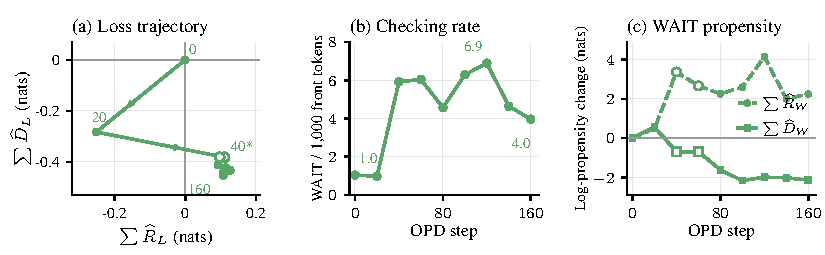
\includegraphics[width=\linewidth]{figures/section33/rd_prepared.pdf}
\caption{\textbf{Loss and checking during the prepared run.} Left: cumulative routing and drift contributions to local loss. Middle: WAIT-family tokens per thousand response tokens, measured in the first 512 tokens. Right: cumulative routing (dashed) and drift (solid) of mean log-WAIT probability at candidate sentence starts in the same window. The last panel decomposes log probability, which is distinct from emitted frequency. Open markers denote substituted evaluator checkpoints.}
\label{fig:rd-prepared-full}\label{fig:rd-prepared}
\end{figure}

The WAIT emission rate also rises and then falls (\cref{fig:rd-prepared-full}, middle). To see whether the model changes its predictions on the same prefixes, we evaluate each checkpoint on the candidate sentence starts in the first 512 tokens of batch 41 (\cref{fig:rd-prepared-audit}, left). Mean WAIT probability rises from $0.0494$ at checkpoint 20 to $0.1130$ at checkpoint 50. It then falls to $0.0842$ at checkpoint 100 and is $0.0874$ at checkpoint 160. The later decrease therefore includes a change in predictions on unchanged prefixes. The probability remains above its level at checkpoint 20.

Mean log-WAIT probability gives another view of the change across rollout batches (\cref{fig:rd-prepared-full}, right). Drift is positive in the first comparison ($+0.56$) and negative by checkpoint 50 ($-1.25$). Routing is positive during the expansion ($+2.89$). Further decreases from drift accumulate through checkpoint 100. Later changes, including much of the decline between batches 121 and 141, mainly come from prefix visitation. These contributions sum to a change in mean log probability, not in emitted frequency. On some other fixed prefix sets, mean log probability and arithmetic mean probability change in opposite directions. We therefore keep these measurements separate.

\begin{figure}[ht]
\centering
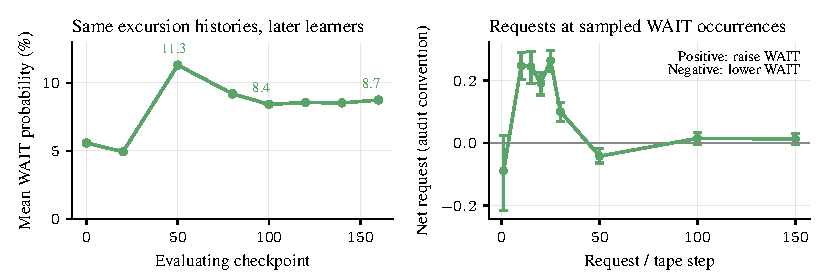
\includegraphics[width=\linewidth]{figures/section33/rd_support_prepared.pdf}
\caption{\textbf{Changes on fixed prefixes and changes in teacher requests.} Left: mean WAIT probability at the same sentence starts in the first 512 tokens of batch-41 rollouts, evaluated by each checkpoint. Right: mean request at sampled WAIT occurrences before an answer in full training batches, with the reported 95\% intervals. Positive requests favor the sampled WAIT token; negative requests suppress it. The two panels use different prefix sets.}
\label{fig:rd-prepared-audit}
\end{figure}

\paragraph{How the teacher's requests change.}
Overall, the requests change from favoring WAIT to suppressing it on average. More specifically, we examine requests at sampled WAIT occurrences in full training batches (\cref{fig:rd-prepared-audit}, right). The mean request is about $+0.19$ to $+0.26$ at batches 10--25, with intervals above zero. At batch 50, it is $-0.0418$ (95\% interval $[-0.0635,-0.0182]$), and $0.528$ of the sampled requests are negative. Later means are nearer zero. 

\Needspace{9\baselineskip}
\paragraph{Remaining calibration errors.}
We finally ask whether these changes bring checking probabilities closer to the teacher's. The prefix classes are fixed at checkpoint 20, and we compare checkpoints 20 and 200 on the same pooled prefix set (\cref{tab:rd-check-calibration}). The discrepancy increases from $0.0276$ to $0.0580$ in the above-teacher class. It decreases from $0.5627$ to $0.3813$ in the below-teacher class. On average, calibration improves only in the initially below-teacher class.

Over-use also grows within the above-teacher subset with $q_W\ge0.05$. Mean student probability rises approximately $0.33\to0.50$ on its own text and $0.29\to0.46$ on held-out text, against teacher probability about $0.15$. The changes still depend on teacher probability after accounting for the reference student's probability, including on held-out prefixes. Thus the student's adjustments remain related to the teacher, but the calibration improvement appears imperfect and weaker than the DeepSeek run.

\FloatBarrier
\Needspace{10\baselineskip}
\subsection{Uncertainty across rollout depths}
\label{app:rd-sensitivity}\label{app:broadcast-evidence}

We next examine when uncertainty rises and where it appears in the response. \Cref{fig:broadcast-onset} uses full training batches from the unprepared Qwen run. Each training update samples 256 rollouts on DAPO prompts at temperature one, with an 8,192-token generation cap.

The left heatmap reports student surprisal: the negative log probability of the token the student generated. The right heatmap reports the teacher's highest next-token probability at the same prefix. Surprisal uses the sampled token, whereas the entropy measurements above use the full next-token distribution. The heatmaps summarize 512-token windows. Rows index rollout batches, including those labeled ``tape step'' in the main figure. Batch $\ell$ follows $\ell-1$ updates. Hatched cells and table dashes indicate that no value is reported there, as the model does not reach that generation length yet.

\begin{figure}[ht]
\centering
\begin{subfigure}{.49\linewidth}
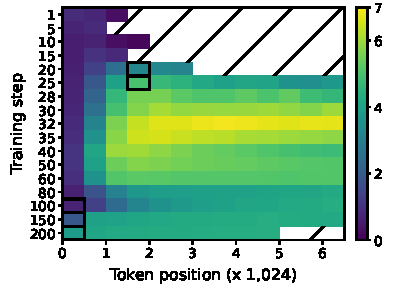
\includegraphics[width=\linewidth]{figures/fig_broadcast_entropy_heatmap.pdf}
\caption{Student surprisal for sampled tokens.}\label{fig:broadcast-entropy}
\end{subfigure}\hfill
\begin{subfigure}{.49\linewidth}
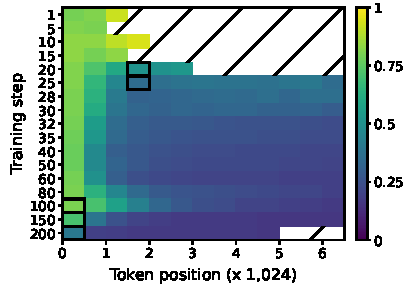
\includegraphics[width=\linewidth]{figures/fig_broadcast_teacher_heatmap.pdf}
\caption{Teacher top-1 probability.}\label{fig:broadcast-teacher}
\end{subfigure}
\caption{\textbf{Uncertainty at different response depths during training.} Student surprisal and teacher top-1 probability are measured on the same student-generated prefixes, in 512-token windows. Hatched cells have no reported value. The plots describe the observed training trajectory.}\label{fig:broadcast-onset}
\end{figure}

\Cref{tab:broadcast-onset} gives two example windows. Between batches 20 and 35, surprisal at positions 1536--2047 rises from $3.24$ to $6.47$ nats. In the first 512 tokens, it rises only from $0.62$ to $0.90$. Teacher top-1 probability falls from $0.51$ to $0.29$ in the deeper window, compared with $0.81$ to $0.78$ in the front window. Thus the early increase in uncertainty is much larger in the deeper of these two windows. The change is not monotone: deep-window surprisal falls to $3.19$ by batch 100. Our main routing and drift analysis ends at batch 161.

\begin{table}[ht]
\centering\small
\setlength{\tabcolsep}{6pt}
\begin{tabular}{r rr rr}
\toprule
&\multicolumn{2}{c}{Student surprisal (nats)}&\multicolumn{2}{c}{Teacher top-1 probability}\\
\cmidrule(lr){2-3}\cmidrule(lr){4-5}
Batch & First 512 & 1536--2047 & First 512 & 1536--2047\\
\midrule
1 & .85 & --- & .79 & ---\\
5 & .69 & --- & .81 & ---\\
10 & .58 & .12 & .83 & .94\\
15 & .58 & --- & .83 & ---\\
20 & .62 & 3.24 & .81 & .51\\
25 & .66 & 4.97 & .81 & .35\\
28 & .70 & 5.55 & .80 & .31\\
30 & .74 & 5.71 & .80 & .33\\
32 & .83 & 6.38 & .79 & .30\\
35 & .90 & 6.47 & .78 & .29\\
40 & 1.04 & 6.00 & .77 & .27\\
50 & 1.05 & 5.69 & .77 & .27\\
60 & .95 & 5.20 & .79 & .24\\
80 & .65 & 3.70 & .80 & .34\\
100 & .66 & 3.19 & .80 & .43\\
150 & 1.89 & 4.14 & .71 & .20\\
200 & 3.85 & 4.26 & .40 & .17\\
\bottomrule
\end{tabular}
\caption{\textbf{Two response windows from the heatmaps.} The first column gives the rollout batch. Batch $\ell$ is generated after $\ell-1$ updates. Student values are sampled-token surprisal. A dash indicates no reported value.}
\label{tab:broadcast-onset}
\end{table}

% Supplement for Appendix E (sec_app_routing_drift.tex).
% Prose paragraphs are stored as single source lines, without manual breaks.
%
% PROVENANCE / INTEGRATION NOTES:
% The continuation design and rounded contrasts were supplied in the editing conversation. The original Overleaf archive contains neither the raw continuation records nor the aggregate export. These are transcribed point estimates, not a new computation from raw outcomes.
% Confirm decoder settings, stopping rules, inherited-prefix serialization, total-budget handling, and grader implementation against the experiment records. No settings or uncertainty intervals were inferred from the separate answer-boundary study.
% In particular, verify that the exported averages retain earlier terminal responses with their original scores and the full rollout-bank denominator. A mean conditional on surviving to the cut is a different quantity.

\newpage
\subsection{Fixed-reference continuation experiments}
\label{app:continuation-profile}
\label{app:fixed-reference-continuations}

The answer-versus-continue experiment in \cref{app:steer-probe} conducted a case study probing continuation from fixed prefixes. This, however, is not enough in understanding the decline in terminal score of the trained student model. Recall that, at a high level, the broadcast not only affects continuation behaviors of the model, but also changes its prefix visitation probabilities. Therefore, to understand the terminal-score decline during OPD, we must also consider how the prefixes that the student checkpoints generates as training proceeds. At any rollout depth, successful completion depends on two quantities: which prefixes the student reaches, and how successfully it continues from those prefixes. We first express terminal score in terms of these two quantities, then show how the reference-policy experiment separates their changes.

\paragraph{Prefix visitation and continuation.}
Fix a cut depth $h$. Recall our notation from before, that $d_t(x)$ is the probability that checkpoint $t$ reaches prefix $x$, and $V_t^Y(x)$ is its expected terminal score when it completes that prefix. The set of rollout cuts $\mathcal C_h$ includes depth-$h$ prefixes and responses that ended earlier (an earlier \emph{completed} response just retains its terminal score). Conditioning on $\mathcal C_h$ gives
\[
 J_Y(t)=\sum_{x\in\mathcal C_h}d_t(x)V_t^Y(x).
\]
This is just the usual average over the ``continuation problems'' presented to the student by its own generation. Training changes both the weights $d_t$ and the continuation values $V_t^Y$. Comparing each checkpoint's prefixes using that checkpoint as the continuer therefore only measures their \emph{combined} effect.

\paragraph{Hold the continuer fixed.}
Using the initial student as the reference, add and subtract $\sum_{x\in\mathcal C_h}d_t(x)V_0^Y(x)$ to obtain
\begin{equation}
 \begin{aligned}
 J_Y(t)-J_Y(0)
 &=\underbrace{\sum_{x\in\mathcal C_h}[d_t(x)-d_0(x)]V_0^Y(x)}_{\text{prefix visitation, evaluated by the initial continuer}}
 \quad+\underbrace{\sum_{x\in\mathcal C_h}d_t(x)[V_t^Y(x)-V_0^Y(x)]}_{\text{continuation change on the same current prefixes}}.
 \end{aligned}
 \label{eq:continuation-reference-split}
\end{equation}
The first term \emph{compares the initial and trained prefix distributions} while keeping the continuer fixed. A negative value means that the initial student finds the trained prefixes harder to finish than its own prefixes. The second term keeps the trained prefix distribution fixed and compares the two continuers. A negative value means that the trained student is less successful than the initial student on those same prefixes. Thus the comparison changes the prefix-generating policy first, then the continuing policy.

Our experiment implements the intermediate case directly: checkpoint $t$ generates the first $h$ tokens, and the initial student completes the rest of the rollout. Let us write its expected score as
\begin{equation}
 F_t^0(h)=\sum_{x\in\mathcal C_h}d_t(x)V_0^Y(x).
 \label{eq:continuation-handoff}
\end{equation}
The two terms in \cref{eq:continuation-reference-split} are therefore $F_t^0(h)-J_Y(0)$ and $J_Y(t)-F_t^0(h)$. They can be estimated by averaging completed responses. The first supplies a common measure of prefix difficulty across checkpoints; the second compares continuers on each checkpoint's own prefix distribution. 

\paragraph{Experimental setup and results.}
The study uses 250 held-out MATH problems, two source rollouts per problem from each of checkpoints 50, 100, and 200, and cuts at 256, 512, and 1,024 response tokens. Each active prefix is continued four times by the generating checkpoint, the initial student, and the teacher. All continuers receive the remainder of an 8,192-token total response budget. The readout is extracted-answer success on the full prefix and continuation; the answer need not be immediately followed by an end-of-turn token. Stopping is recorded separately. The estimator averages continuation scores within each prefix, then over the two source rollouts and uniformly over problems, retaining earlier completed responses as above. This population and budget differ from those of the selected answer-boundary probe in \cref{app:steer-probe}. The reported values below are rounded sample means; independently sampled self-continuations estimate the same $J_Y(t)$ but need not give identical means at different cuts.
% This experiment does not inherit T=0.6, top-p=0.95, or the 16,384-new-token budget from app:steer-probe. Raw records are needed to verify the aggregation convention and estimate uncertainty while preserving prompt and prefix pairing.

Consider the 256-token cut at step 50. The initial student scores $48.4\%$ on its own rollouts and $50.5\%$ when it completes the trained checkpoint's prefixes. The trained checkpoint scores $39.5\%$ on those same prefixes. The first comparison therefore contributes $+2.1$ percentage points, while the second contributes $-11.0$ points, accounting for the total $-8.9$-point difference. At this cut, the prefixes remain usable by the initial student; the trained student loses performance in completing them.

\begin{table}[ht]
\centering\small
\setlength{\tabcolsep}{8pt}
\begin{tabular}{r rrr}
\toprule
Cut depth & Step 50 & Step 100 & Step 200\\
\midrule
256   & $+2.1$ & $-1.7$ & $-5.9$\\
512   & $-1.3$ & $-2.7$ & $-6.1$\\
1,024 & $-8.1$ & $-7.6$ & $-8.5$\\
\bottomrule
\end{tabular}
\caption{Change in initial-policy completion success, $100[F_t^0(h)-J_Y(0)]$, in percentage points. The initial student completes prefixes from each trained checkpoint; its own-rollout baseline is $48.4\%$. These are the values plotted in \cref{fig:rd-initial-continuation}, reported as rounded aggregate point estimates from one training run.}
\label{tab:continuation-reference}
\end{table}

\Cref{tab:continuation-reference} shows that at step 50, the initial continuer already scores lower on deep prefixes: the 1,024-token contrast is $-8.1$ points. At later checkpoints, the deficit also reaches the shallow cuts, while the 1,024-token deficit remains similar in magnitude. On the 256-token prefixes, the trained-minus-initial continuation contrast remains negative at steps 100 and 200 ($-12.1$ and $-6.2$ points). By step 200, both terms in \cref{eq:continuation-reference-split} are negative: the initial student finds the new prefixes harder, and the trained student completes those prefixes less successfully than the initial student.

\paragraph{Connection to \Cref{eq:broadcast-continuations}.}
The same two factors describe the instantaneous dynamics. Differentiating the cut identity gives
\begin{equation}
 \dot J_Y(t)=\sum_{x\in\mathcal C_h}\dot d_t(x)V_t^Y(x)+\sum_{x\in\mathcal C_h}d_t(x)\dot V_t^Y(x).
 \label{eq:continuation-infinitesimal}
\end{equation}
Under the regularity assumptions in \cref{prop:rd-value-cut}, the first term computes the contributions to \cref{eq:broadcast-continuations} from decisions before the cut, and the second collects those from the cut onward. Both arise from the same shared parameter update. If the reference is checkpoint $t$ instead of checkpoint 0, and the compared policy is an infinitesimally later checkpoint $t+dt$, the differences in \cref{eq:continuation-reference-split} (divided by elapsed training time) recover the derivative, hence recovering these two terms. Such measurements are unrealistic to implement and too noisy to measure in practice, however, so our experiment instead use the initial policy as the reference continuer to magnify the trend of visited-prefix quality / continuation difficulty.

\paragraph{What does moving the cut measure?}
Another interesting question is, at a fixed checkpoint $t$, moving the rollout cut from $h_1$ to $h_2$ lets the trained student generate an additional block of tokens before the initial student takes over. A decrease in $F_t^0$ means that this additional trained-student generation leaves the initial continuer less able to reach a correct answer. To connect it to continuation advantages, let us follow the initial student's value along a trained rollout. For each action decision, $\mathcal A_0^Y(x_j,a_j)=V_0^Y(x_{j+1})-V_0^Y(x_j)$. Summing over a block yields a telescoping series over depth of the cuts, then averaging over the rollouts gives
\begin{equation}
 F_t^0(h_2)-F_t^0(h_1)=\sum_{\substack{x\in\mathcal S\\h_1\le h(x)<h_2}}d_t(x)\Ex_{a\sim\pi_t(\cdot\mid x)}[\mathcal A_0^Y(x,a)].
 \label{eq:continuation-block-identity}
\end{equation}
Here $\mathcal S$ contains decision prefixes; completed responses contribute no further decisions and retain their scores. At depth zero, the initial student generates the whole response, so $F_t^0(0)=J_Y(0)$. At the total response cap, the trained student has generated the whole response, so $F_t^0(H_{\max})=J_Y(t)$. Consequently, the differences across any partition of the full response sum to $J_Y(t)-J_Y(0)$. Fixed cuts therefore measure aggregate contributions of token blocks to this finite policy comparison, using completed outcomes in place of separate continuation-value estimates at every token.
